\documentclass{beamer}

%Packages BEGIN
\usepackage{amsmath}
\usepackage{xeCJK} % use this package to set Chinese and English font separately
\usepackage{fontspec} 
\usepackage{listings}
\usepackage{xcolor}
 
 

%Packages END

%Style setting BEGIN
\usetheme{Madrid} 
\usecolortheme{default} 
\definecolor{codegreen}{rgb}{0,0.6,0}
\definecolor{codegray}{rgb}{0.5,0.5,0.5}
\definecolor{codepurple}{rgb}{0.58,0,0.82}
\definecolor{backcolour}{rgb}{0.95,0.95,0.92}
 
\lstdefinestyle{mystyle}{
    backgroundcolor=\color{backcolour},   
    commentstyle=\color{codegreen},
    keywordstyle=\color{magenta},
    numberstyle=\tiny\color{codegray},
    stringstyle=\color{codepurple},
    basicstyle=\ttfamily\footnotesize,
    breakatwhitespace=false,         
    breaklines=true,                 
    captionpos=b,                    
    keepspaces=true,                 
    numbers=left,                    
    numbersep=5pt,                  
    showspaces=false,                
    showstringspaces=false,
    showtabs=false,                  
    tabsize=2
}
 
\lstset{style=mystyle} 

% Serif font in Ubuntu. Choose the Chinese font available in your device
\setCJKmainfont{Noto Serif CJK TC}

% Serif font in Ubuntu. Choose the Chinese font available in your device
\setCJKmonofont{Noto Serif CJK TC}

% Serif font in Ubuntu. Choose the Chinese font available in your device
\setCJKsansfont{Noto Serif CJK TC}

\XeTeXlinebreaklocale "zh" % enabling auto linebreaks
\XeTeXlinebreakskip = 0pt plus 1pt % enabling auto linebreaks
 
%Style setting END


\begin{document}

\frame{\titlepage} 

\begin{frame}[fragile]
some text
\begin{lstlisting}[language=python]
print('fuck')
\end{lstlisting}
\end{frame} 

\begin{frame}
	\frametitle{Image Recognization}
	\textbf{Goal}: Indentify words in a picture and generate flashcards.
	\begin{figure}[h]
		\centering
		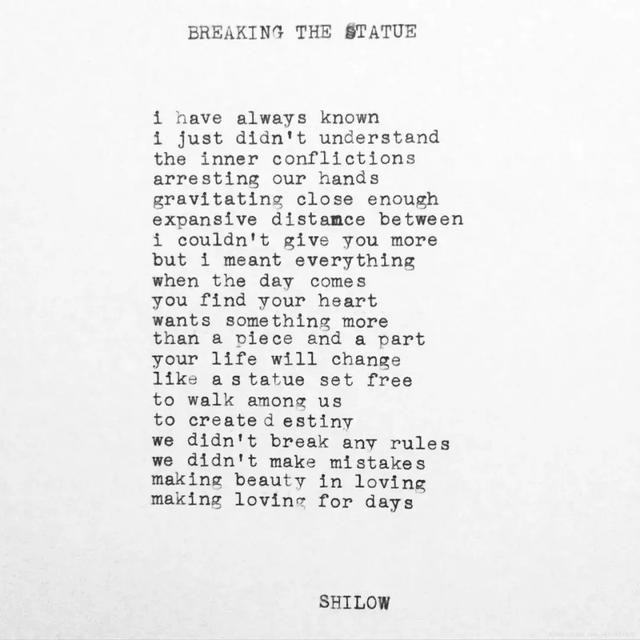
\includegraphics[width=0.55\linewidth]{./img1.jpg}
		\caption{Target picture}
	\end{figure}
\end{frame}

\begin{frame}{Method}
		\textbf{Step 1}: Convert the picture to grayscale, then set the darker pixels to absolute black, lighter pixels to absolute white.\\
		\textbf{Step 1-1}: To implement Step 1, we turn the picture into np.arrays.
		%\begin{figure}[h]
			%\centering
			%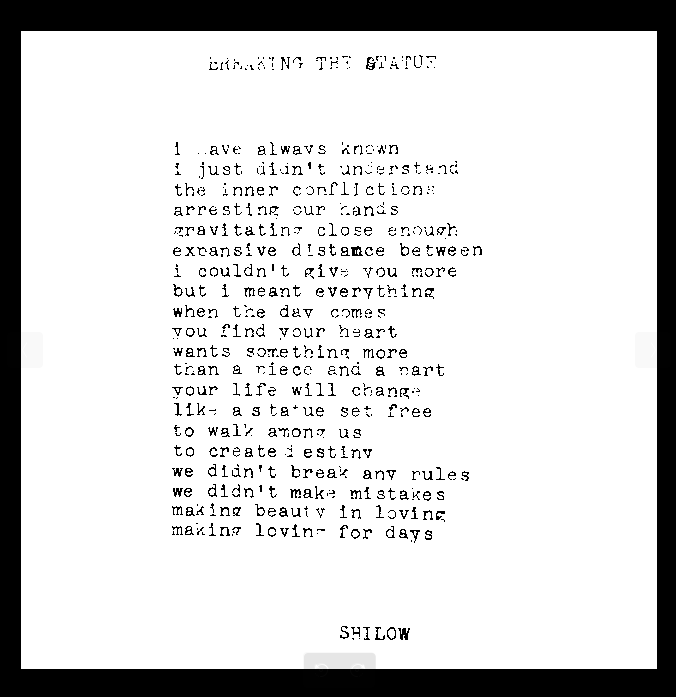
\includegraphics[width=0.50\linewidth]{./picture_blackwhite.png}
		%\end{figure}
\end{frame}

\begin{frame}{Task}
		\textbf{How do computers recognize a word?}
		\begin{figure}[h]
			\centering
			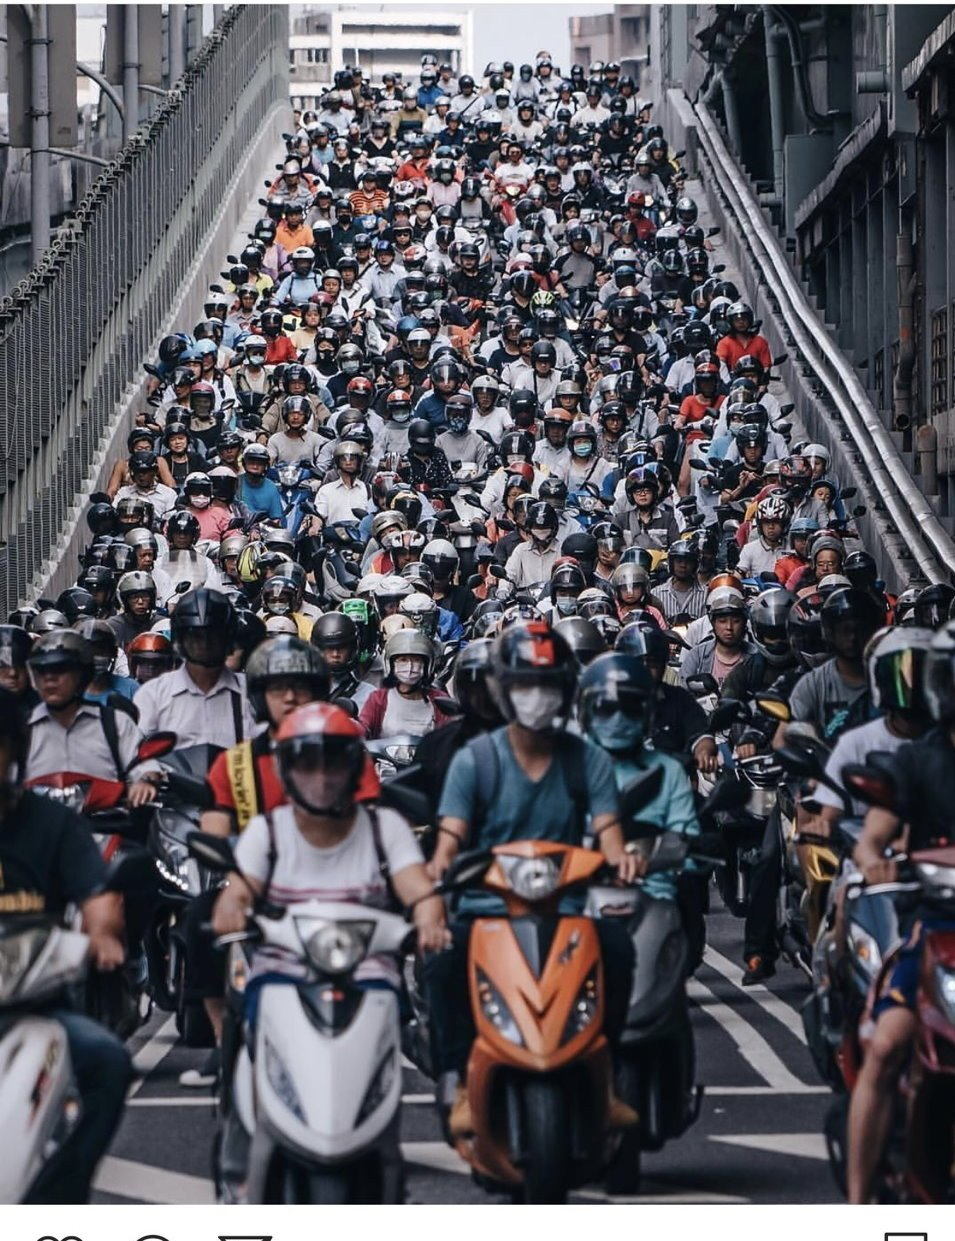
\includegraphics[width=0.55\linewidth]{./motor.jpg}
		\end{figure}
\end{frame}

\begin{frame}{Fourier Transform}
	\textbf{Seems good...but does it?}
		\begin{figure}[H]
			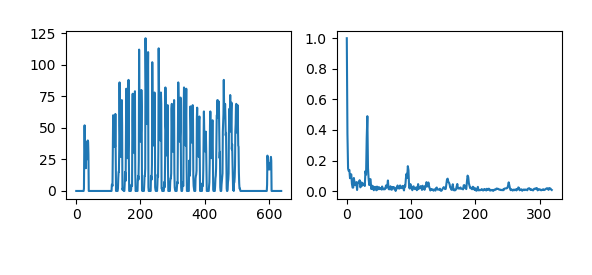
\includegraphics[width=0.45\linewidth]{./fourier.png}
			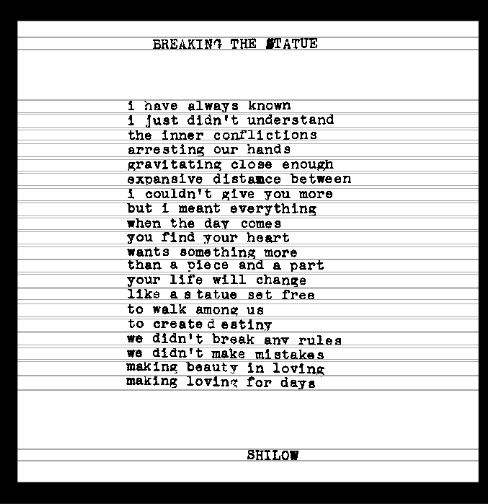
\includegraphics[width=0.55\linewidth]{./imgslice.png}
		\end{figure}
\end{frame}

\begin{frame}{Fourier Transform}
	\textbf{Fewer data lead to less precision.}
	\begin{figure}[H]
		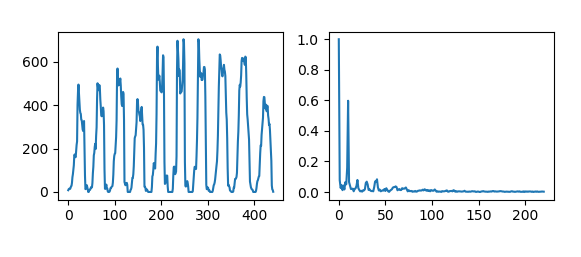
\includegraphics[width=0.55\linewidth]{./fourier2.png}
		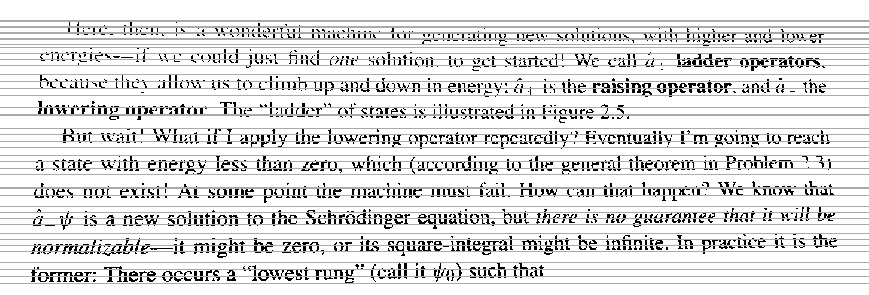
\includegraphics[width=0.70\linewidth]{./imgslice2.png}
	\end{figure}
\end{frame}

\begin{frame}{Method}
	\textbf{Step 2-1}: When the number of black pixels on a row (of pixels) is below a threshold, the row is recognized as the boundary of the line.\\
		\textbf{Step 2-2}: Detect the wider white columns to identify words.\\
		\begin{figure}[h]
			\centering
			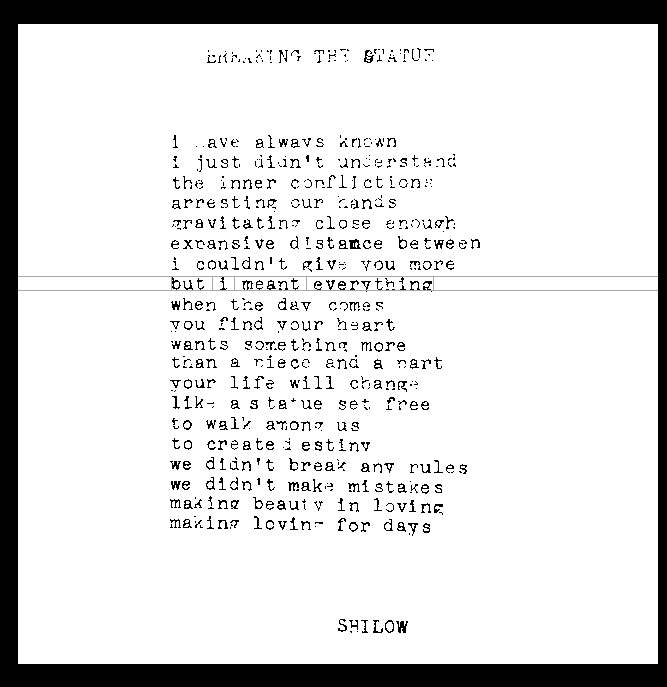
\includegraphics[width=0.50\linewidth]{./raw_done.png}
		\end{figure}
\end{frame}

\begin{frame}{Method}
		\textbf{Step 3-1}: Detect the words in the line, use the order to determine which word I selected. We get WordFromLine.\\
		\textbf{Step 3-2}: Detect the word in the region I selected. We get WordFromWord.\\
		\textbf{Step 3-3}: If the WordFromLine is similar to WordFromWord or len(WordFromWord)=0, return WordFromLine. Else, return WordFromWord.\\
		\begin{figure}[h]
			\centering
			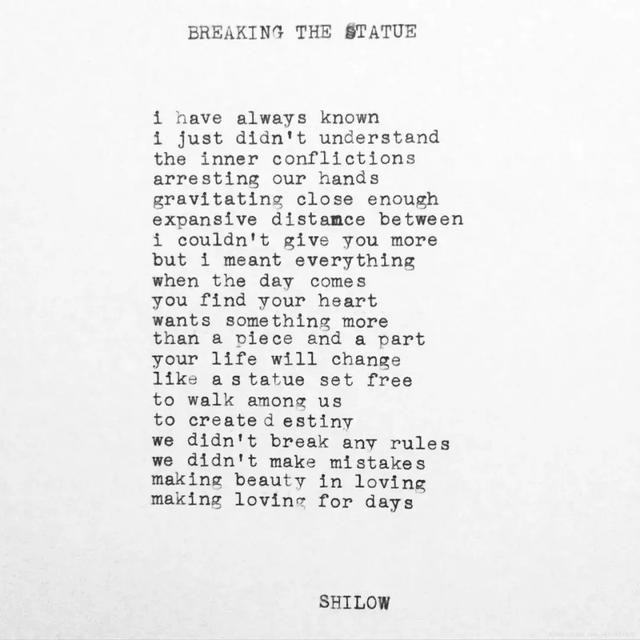
\includegraphics[height=0.4\linewidth]{./img1.jpg}
			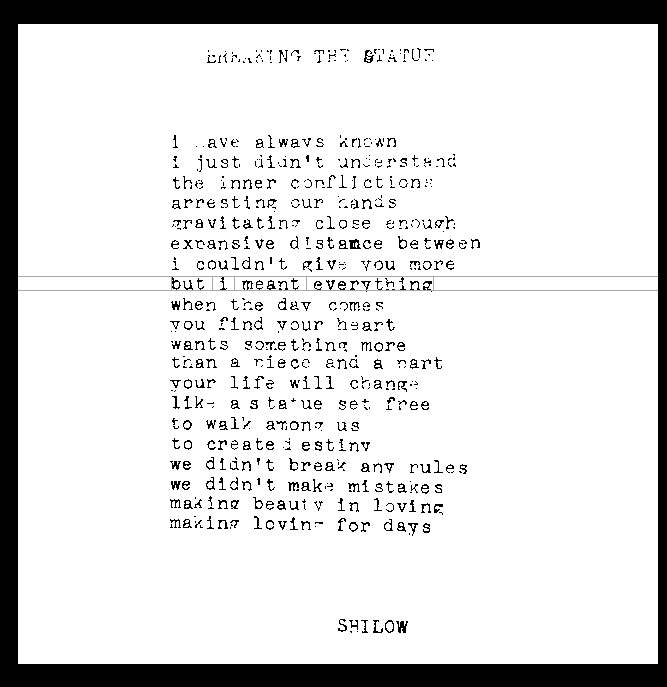
\includegraphics[width = 0.4\linewidth]{./raw_done.png}
		\end{figure}
\end{frame}

\end{document}
